\chapter{Introducción}

Cada día, utilizamos aplicaciones de cómputo más complejas que resuelven problemas más complicados, debido a que estos problemas involucran el procesamiento de grandes volúmenes de datos o también involucran la omnipresencia de contenido multimedia; así, éstas aplicaciones demandan cada vez más poder de cómputo. Por ejemplo, hay instituciones financieras que necesitan procesar millones de transacciones diariamente; así, utilizan aplicaciones que durante el día guardan las operaciones bancarias y en la noche ejecutan estas operaciones en lotes para actualizar las cuentas bancarias. En la Bolsa Mexicana de Valores, el motor de negociación transaccional, MoNeT, puede procesar hasta 100,000 transacciones por segundo \cite{bmv2012informe}. 

Otro ejemplo son las películas de animación: cuando los diseñadores han terminado de modelar a los personajes junto con el entorno y cuando también han especificado las animaciones de los personajes sobre el entorno, se requiere generar cada fotograma de la animación para después juntarlos y proyectarlos rápidamente para crear la ilusión de movimiento y, de esta forma, crear una película. Por ejemplo, en el 2005, investigadores de la Universidad de Innsbruck en Austria generaron una animación tridimensional, primero utilizando una sola computadora y luego utilizando varias computadoras interconectadas \cite{nerieri2005using}. En el primer caso, tardaron aproximadamente 6 días en procesar la animación cuya duración es de un minuto. Por otro lado, utilizando varias computadoras, la animación fue procesada en poco menos de una hora.

Un último ejemplo son los proyectos de cómputo científico: éstos requieren hacer numerosos cálculos para llegar a resultados pertinentes. Tal es el caso del descubrimiento del bosón de Higgs en el Gran Colisionador de Hadrones (LHC) de la Organización Europea para la Investigación Nuclear (CERN). Se estima que cada año, el detector principal del LHC genera 15 petabytes (aproximadamente $15 \times 10^{15}$ bytes) de datos que requieren ser analizados \cite{shiers2007worldwide}. 

¿Qué tienen en común todas estas aplicaciones? Para empezar, toman mucho tiempo en ejecutarse. Entonces, una posible solución para disminuir el tiempo de ejecución de estas aplicaciones es distribuir el gran trabajo que requieren estos proyectos entre varias computadoras. Para ello, necesitamos dividir nuestra aplicación en partes más pequeñas e independientes, algunas de ellas podrán ejecutarse de manera concurrente y paralela, otras no. De esta forma, tendríamos una solución escalable, es decir, si aumentamos el número de computadoras disponibles para nuestra aplicación, reduciremos el tiempo de ejecución.

Lograr esta paralelización requiere un esfuerzo por parte del desarrollador de la aplicación. Existen técnicas de paralelización que permiten al desarrollador expresar la aplicación en varias partes paralelas. A continuación, enlistaremos algunas de estas técnicas:

\begin{itemize}
\item{\textbf{Programas multiproceso.} En esta técnica, la idea principal es utilizar varios procesos para repartir el cómputo. Por ejemplo, en el modelo fork/join, un programa se invoca recursivamente a sí mismo (fork), de tal modo que cada subprograma resuelve un problema más pequeño que el problema original. Después, los resultados parciales de cada subprograma son juntados en un sólo programa (join).}

\item{\textbf{Threads.} Un proceso, en vez de invocarse a sí mismo varias veces, también puede invocar \emph{threads} o hilos de ejecución que, a diferencia de un proceso, éstos no son controlados por el administrador de procesos del sistema operativo, sino por el programa mismo. Por lo tanto, ocupan menos recursos del sistema. De igual modo, se pueden implementar varios modelos de programación concurrente (fork/join o productor/consumidor, como ejemplos) como se hacen con los programas multiproceso.}

\item{\textbf{MapReduce.} Este paradigma de programación especializado en procesar grandes volúmenes de datos \cite{dean2008mapreduce} funciona de la siguiente forma: primero se define una función $map(): (k_1,A) \rightarrow list(k_2,B)$, que se aplica a todos los elementos de tipo $A$ para asociarles una llave y transformarlos al tipo $B$. Luego, la función $reduce(): (k_2, list(B)) \rightarrow list(B)$, hace alguna operación asociativa para sumarizar los resultados.}

\item{\textbf{MPI.} La interfaz de paso de mensajes (MPI por sus siglas en inglés) es un conjunto de definiciones de bibliotecas \cite{lusk2009mpi}, cuyas subrutinas son utilizadas por varios procesos paralelos para que puedan comunicarse entre si enviándose mensajes de manera asíncrona.}
\end{itemize}

Aunque estas técnicas de paralelización son muy efectivas, éstas son aplicadas cuando el problema a resolver ha sido bien definido y cuando sólo hay una instancia de la aplicación que resuelve el problema planteado. 

Ahora bien, hay aplicaciones que involucran varios pasos que están relacionados entre sí, por ejemplo, que el programa $C$ requiera de la salida del programa $A$ y del programa $B$ para que pueda funcionar, tal y como se muestra en la figura \ref{fig:workflowABC}. También, es conveniente definir los grandes bloques de de la aplicación, porque puede suceder que los programas $A$, $B$ y $C$ están hechos con diferentes técnicas de paralelización y/o construidos con diferentes plataformas y lenguajes, por lo que cada uno debe ejecutarse por separado. 

En los dos casos descritos anteriormente, hay una cierta secuencia que debemos seguir y, dentro de dicha secuencia, hay algunos pasos que podemos resolver de manera concurrente y otros pasos se resuelven de manera secuencial. De esta forma, los pasos de la aplicación representan un \emph{modelo} de nuestro problema.

\begin{figure}
    \begin{center}
        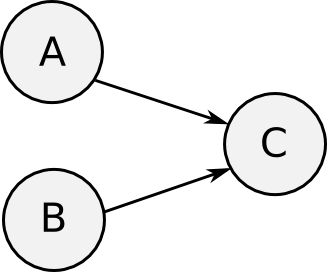
\includegraphics[width=0.25\textwidth]{imagenes/workflowABC}
    \end{center}
    \caption{Flujo de trabajo con una tarea (C) que depende de dos tareas (A y B).}
    \label{fig:workflowABC}
\end{figure}

Este modelo también es llamado \emph{flujo de trabajo}. De manera muy abstracta, un flujo de trabajo es un conjunto de pasos que modelan la ejecución de un proceso. La utilidad de este sencillo concepto ha sido probado en varias áreas, de las cuales mencionaremos dos aplicaciones: en el ámbito de los negocios y en el ámbito científico. 

\begin{itemize}
\item{En el ámbito de los negocios, se puede definir un flujo de trabajo para modelar el proceso de fabricación de un producto. También, es posible expresar un flujo de trabajo con un diagrama dibujado con los bloques y reglas del \emph{Lenguaje de Ejecución de Procesos de Negocio} para después simular su ejecución en una computadora.}

\item{En el ámbito científico, los flujos de trabajo son aplicados para modelar programas que requieran varios pasos para su ejecución. Algunos flujos de trabajo requieren mucho tiempo tiempo de ejecución para la ejecución de sus tareas. Otros flujos de trabajo son muy tienen tareas que tardan poco tiempo en ejecutarse, pero se requieren ejecutar muchas instancias de este flujo de trabajo.}
\end{itemize}

En cualquiera de los dos casos anteriores, es deseable distribuir la ejecución de éstos flujos de trabajo entre varias computadoras. Si bien es posible paralelizar algunos pasos de la ejecución de nuestro flujo de trabajo utilizando las técnicas antes mencionadas, hay restricciones de orden que se deben respetar, por lo cual, es indispensable \emph{planificar} la ejecución del flujo de trabajo entre las múltiples computadoras.

%Hay varias maneras de hacer esta planificac. Cabe aclarar que
%Scheduling is defined as a function that maps each task in a workflow to a service deployed on the Grid that implements this task. The cost model for workflows is described by multiple scheduling criteria
%Definimos la \emph{planificación} como la asignación de recursos con el fin de completar la ejecución de todas las tareas de manera satisfactoria
Definimos la \emph{planificación} como una función que asigna a cada tarea del flujo de trabajo un servicio que contiene los recursos para ejecutar dicha tarea, con el fin de completar la ejecución de todas las tareas de manera satisfactoria, cumpliendo ciertas restricciones \cite{wieczorek2009towards}. Con ello, se desea encontrar una forma óptima de hacer esta planificación, como reducir el tiempo de ejecución total del flujo de trabajo. Sin embargo, con la aparición del cómputo en la nube, es posible ejecutar nuestro flujo de trabajo con otras restricciones, como minimizar el presupuesto necesario para la ejecución del flujo afectando el tiempo de ejecución.

%mencionar instruction level paralelism, data-level parallelism task level paralelism, 

%uml, bepl para software y negocios, buscar los que vienen en el paper de hierarchical scheduling for swindew-c

En este trabajo se hace un estudio de los principales algoritmos de planificación de flujos de trabajo, con énfasis en los algoritmos utilizados en cómputo distribuido, en especial en cómputo en la nube. En el capítulo 2 se provee un estudio detallado del concepto de flujos de trabajo y su aplicación en computación. El capítulo 3 trata los principales enfoques de cómputo distribuido para ejecutar estos flujos. En el capítulo 4 se hace un estudio de los principales algoritmos de planificación de los flujos de trabajo. Finalmente, en el capítulo 6 discutiremos algunas conclusiones sobre el análisis de estos algoritmos.
